\subsection{Syntax-number units interactions}[t]
\lipsum[1]

\begin{figure*}
\centering
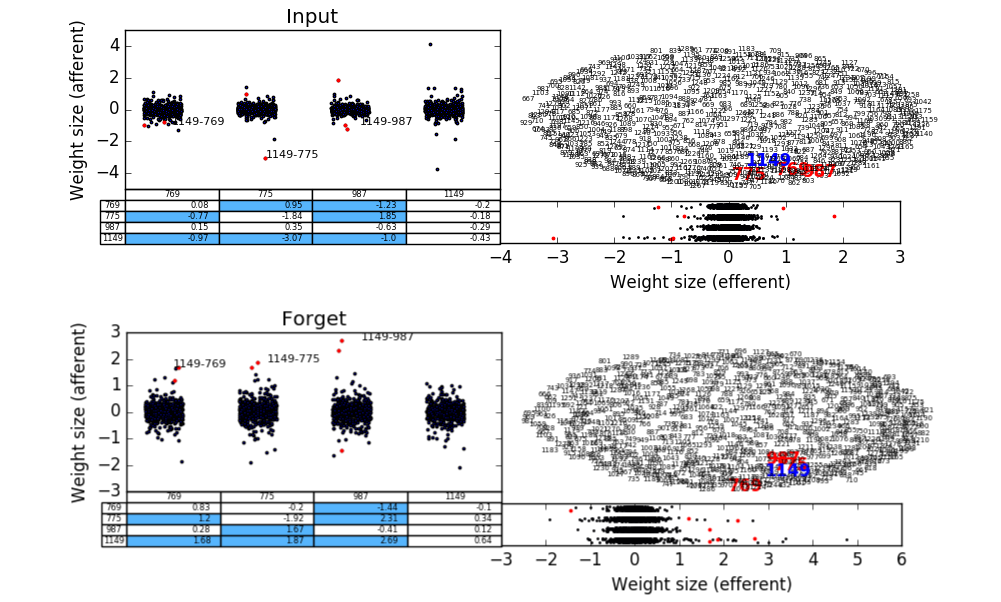
\includegraphics[width=\textwidth]{Figures/Figure7_interactions.png}
\caption{Interaction among the syntax and number units. A value in the table represents the weight size from the unit appearing on the left to the unit appearing on the top row. (A) Distribution of all weight values to the unit appearing on the top row of the table. Outlier weights from the table (more than three standard-deviation above/below the mean) are marked in red; Weight values from the syntax to number units have in addition a corresponding text label. (B) Distribution of all weight values from the unit appearing on the left column of the table. Outlier weights are marked in red. (C)  A visualization of unit interactions. For each gate $g$, an interaction distance $d_{ij}^g$ between a pair of units $i$ and $j$ was first defined as: $d_{ij}^g=exp{-max{w_{ij}^g, w_{ji}^g}}$, where $w_{ij}^g$ is the weight from unit $j$ to the gate $g$ of unit $i$. Then, all interaction distances in the network were visualized using multidimensional scaling. Note that the interaction distances between the number units and between the syntax and number units are relatively close compared to the mean interaction distance in the network.}
\end{figure*}
